% !TEX root = ../../../Masterthesis.tex
\section{Leaving Drydock}\label{sec:leaving drydock}
%-----------------------------------------------------------------------------
% A
%-----------------------------------------------------------------------------
\begin{figure*}[h!]
\center
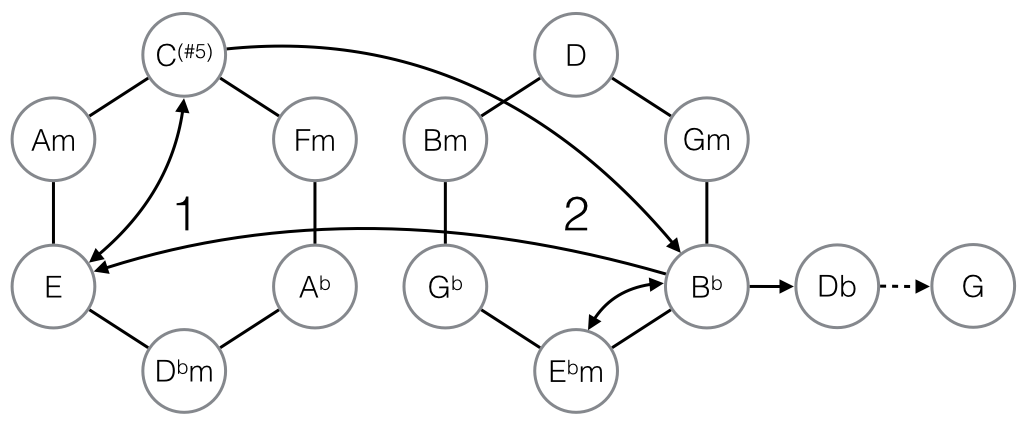
\includegraphics[width=\linewidth]{STTMP_Leaving_Drydock_A}
	\caption{ST:TMP: Leaving Drydock A}
	\label{STTMP_Leaving_Drydock_A}
	%\setfloatalignment{b}
\end{figure*}

\noindent With every crew post now filled, the Enterprise prepares to leave drydock. The music provides an underscore that builds on the tension and excitement that both crew and audience would feel. The time is \lilyTimeSignature{6 + 3}{8 + 4} creating a 3:2 displacement, which Goldsmith uses as a musical device throughout. Goldsmith uses \textbf{N}, thirds and \acf{MTTP}'s to build progressions. See figure \ref{STTMP_Leaving_Drydock_A}. On a few occasions, he uses altered chords and when he does use altered chords there is most likely a \textit{common tone junction} (figure \ref{STTMP_Leaving_Drydock_A2}) binding them together. 

\begin{marginfigure}
%\center
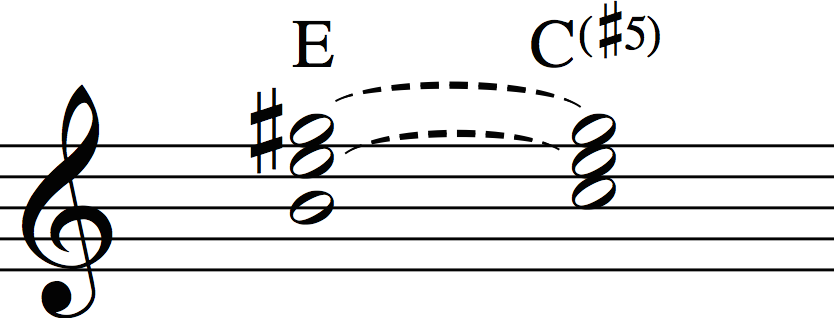
\includegraphics[width=\linewidth]{STTMP_Leaving_Drydock_A2}
	\caption{ST:TMP: Leaving Drydock A: Common Tones}
	\label{STTMP_Leaving_Drydock_A2}
	%\setfloatalignment{b}
\end{marginfigure}

%-----------------------------------------------------------------------------
% B
%-----------------------------------------------------------------------------
\begin{figure}[h!]
\center
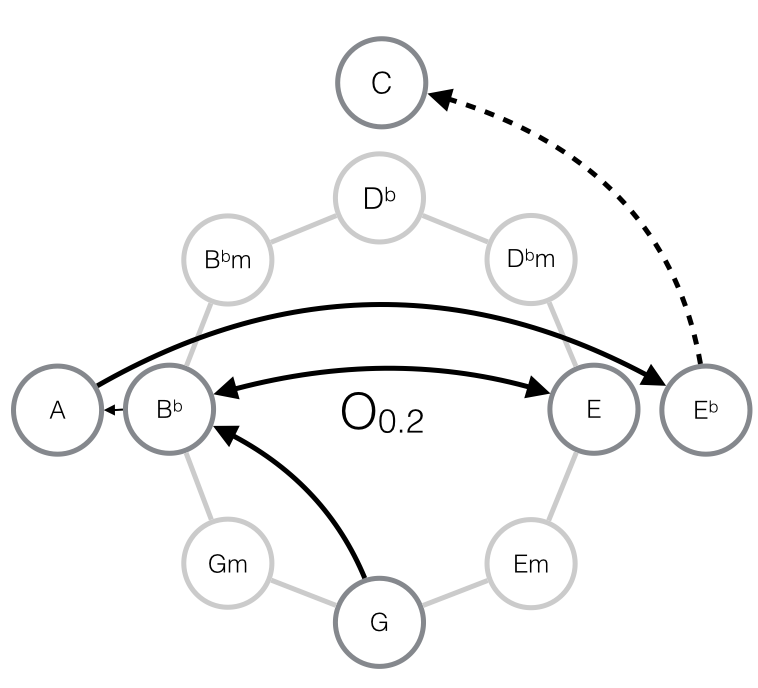
\includegraphics[width=0.8\linewidth]{STTMP_Leaving_Drydock_B}
	\caption{ST:TMP: Leaving Drydock B}
	\label{STTMP_Leaving_Drydock_B}
	\setfloatalignment{b}
\end{figure}
When preparing to exit from the interior to exterior shot, Goldsmith uses a \ac{MTTP} to advance (\textbf{m.23}). When we see the outer hull of Enterprise, Goldsmith uses his Star Trek theme, and does so throughout the score with various treatments. Figure \ref{STTMP_Leaving_Drydock_B} sees \textbf{m.28-30}. It is a three-part trumpet, brassy and pompous, but does not match any significant event on the screen. The harmonic movement however is interesting. Goldsmith moves in minor thirds right up to A, where he makes \textit{chromatic network modulation}. What follows is the Star Trek theme in 3:2 until we cut to the bridge again.

%-----------------------------------------------------------------------------
% D
%-----------------------------------------------------------------------------
\begin{figure}
\center
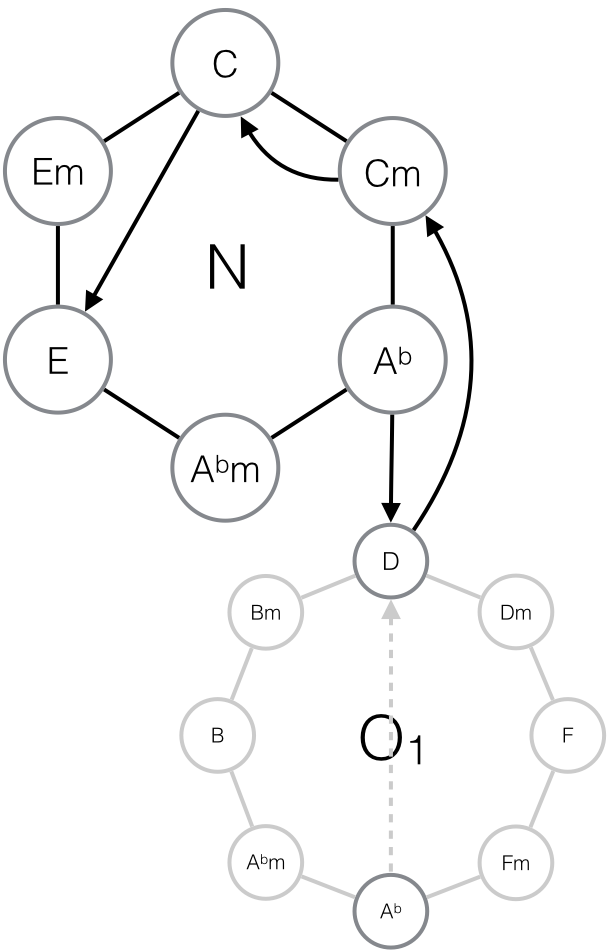
\includegraphics[width=0.6\linewidth]{STTMP_Leaving_Drydock_D}
	\caption{ST:TMP: Leaving Drydock D}
	\label{STTMP_Leaving_Drydock_D}
	\setfloatalignment{t}
\end{figure}
The restless ostinato mimics Kirk, who is clearly electric: ``Thrusters ahead, Mr. Sulu.'' The music builds and the harmonic progression (figure \ref{STTMP_Leaving_Drydock_D}) is as anxious as the captain. This time, the \ac{MTTP} is slightly softened with the incursion of G/B just before \bflat. We once again see the Enterprise, now leaving the drydock, followed by the full version of the Star Trek theme. 

At \textbf{m.72} we are back at the Enterprise, now down in engineering. The restless theme is back, mirroring the people working excitedly. With a new \ac{MTTP} we are out in space again, viewing the Enterprise slowly flying with Earth and the sun as a magnificent backdrop.
%-----------------------------------------------------------------------------
% J
%-----------------------------------------------------------------------------

\begin{marginfigure}[-10cm]
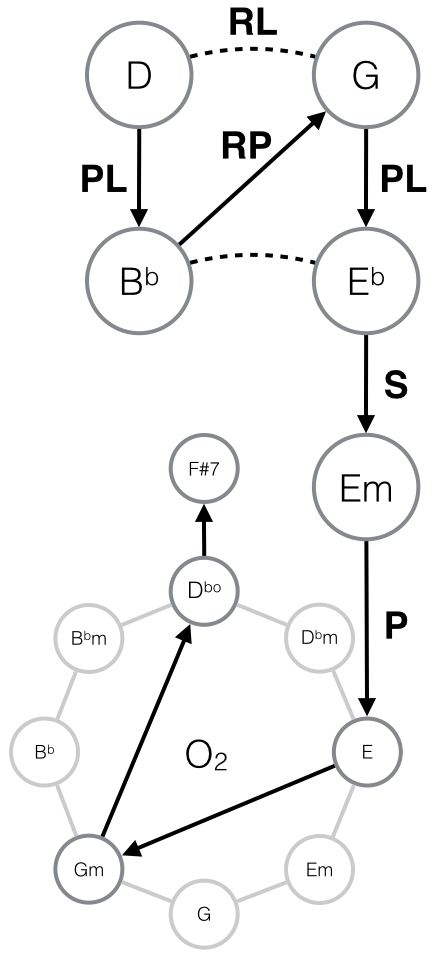
\includegraphics[width=\linewidth]{STTMP_Leaving_Drydock_J}
	\caption{ST:TMP: Leaving Drydock J}
	\label{STTMP_Leaving_Drydock_J}
	\setfloatalignment{b}
\end{marginfigure}

With a small meter change, \lilyTimeSignature{3}{8}, we follow up from last shot down in engineering, figure \ref{STTMP_Leaving_Drydock_J}. Concealed inside the chord progression is the whole tone scale, \textit{pc} [0,2,4,6,8,t],\footnote{\keyboard{C,D,E,Fiss,Giss,Aiss}} figure \ref{STTMP_Leaving_Drydock_J2}, creating a sense of wonder. The progression follows in figure \ref{STTMP_Leaving_Drydock_J}. Goldsmith works through major thirds, connecting them with a minor third, passing on with a \textbf{SLIDE} and continuing with chords with roots that follow minor thirds until \textbf{m.95} where he prepares a \ac{MTTP}, getting there through the two common tones \fiss and \aiss connecting \(D\flatx^{dim}\) and \fiss. After a small 3:2, mixolydian progression reminiscent of the Star Trek theme, we head back out to the Enterprise, now burning her engines to the Star Trek theme \textbf{m.99-103}.

\begin{figure*}
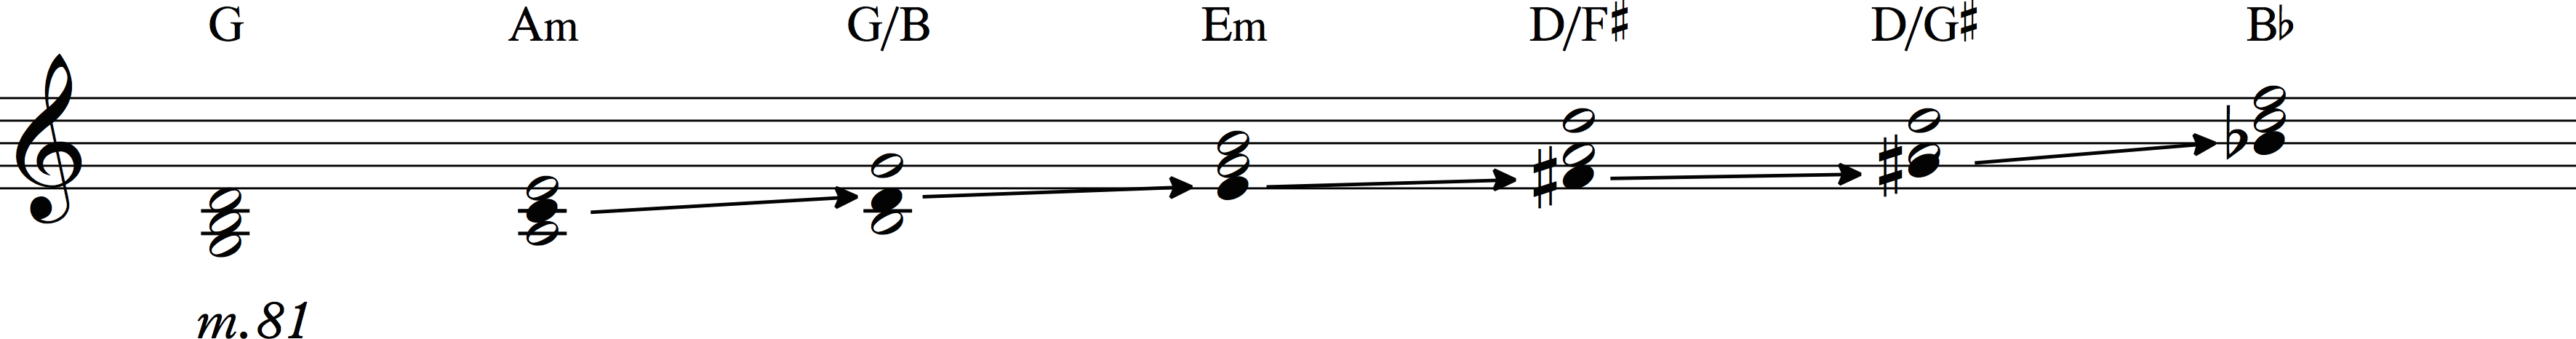
\includegraphics[width=\linewidth]{STTMP_Leaving_Drydock_J2}
	\caption{ST:TMP: Leaving Drydock J: Whole Tone Scale}
	\label{STTMP_Leaving_Drydock_J2}
	\setfloatalignment{b}
\end{figure*}

%-----------------------------------------------------------------------------
% M
%-----------------------------------------------------------------------------
Back inside, the restless theme is repeated once more, continuing the third-progressions, figure \ref{STTMP_Leaving_Drydock_M}. At \textbf{m.111} the captain requests ``Viewer ahead.'' and we get a glimpse of the stars as they pass the ship. Kirk looks outwards proudly while the Star Trek theme plays 3:2. We cut to the outside and the theme returns to its original form as we see the Enterprise rockets past Venus.

\begin{figure}
\center
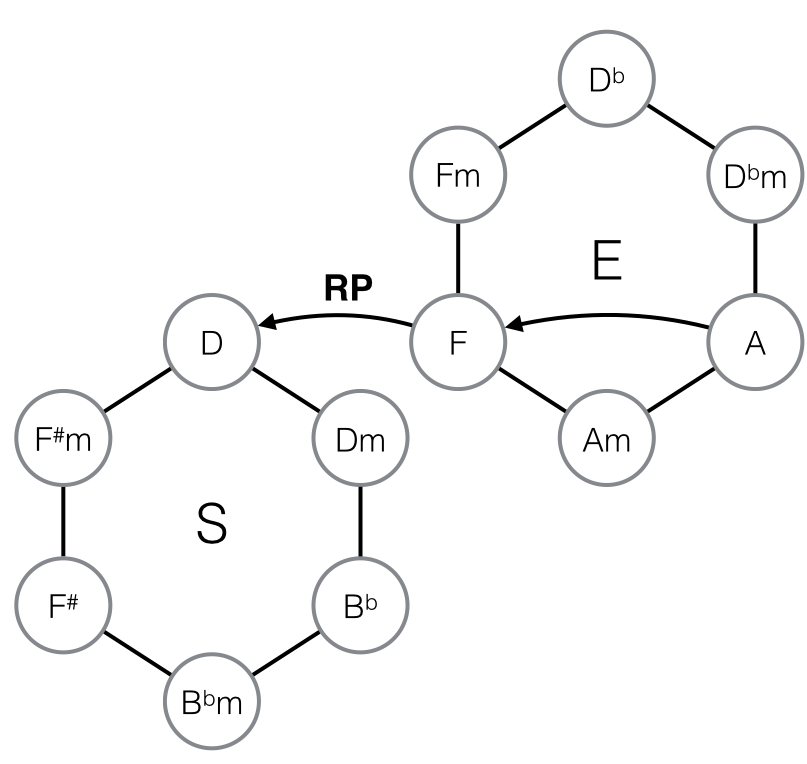
\includegraphics[width=0.8\linewidth]{STTMP_Leaving_Drydock_M}
	\caption{ST:TMP: Leaving Drydock M}
	\label{STTMP_Leaving_Drydock_M}
	\setfloatalignment{b}
\end{figure}


%-----------------------------------------------------------------------------
% PDF
%-----------------------------------------------------------------------------
\clearpage
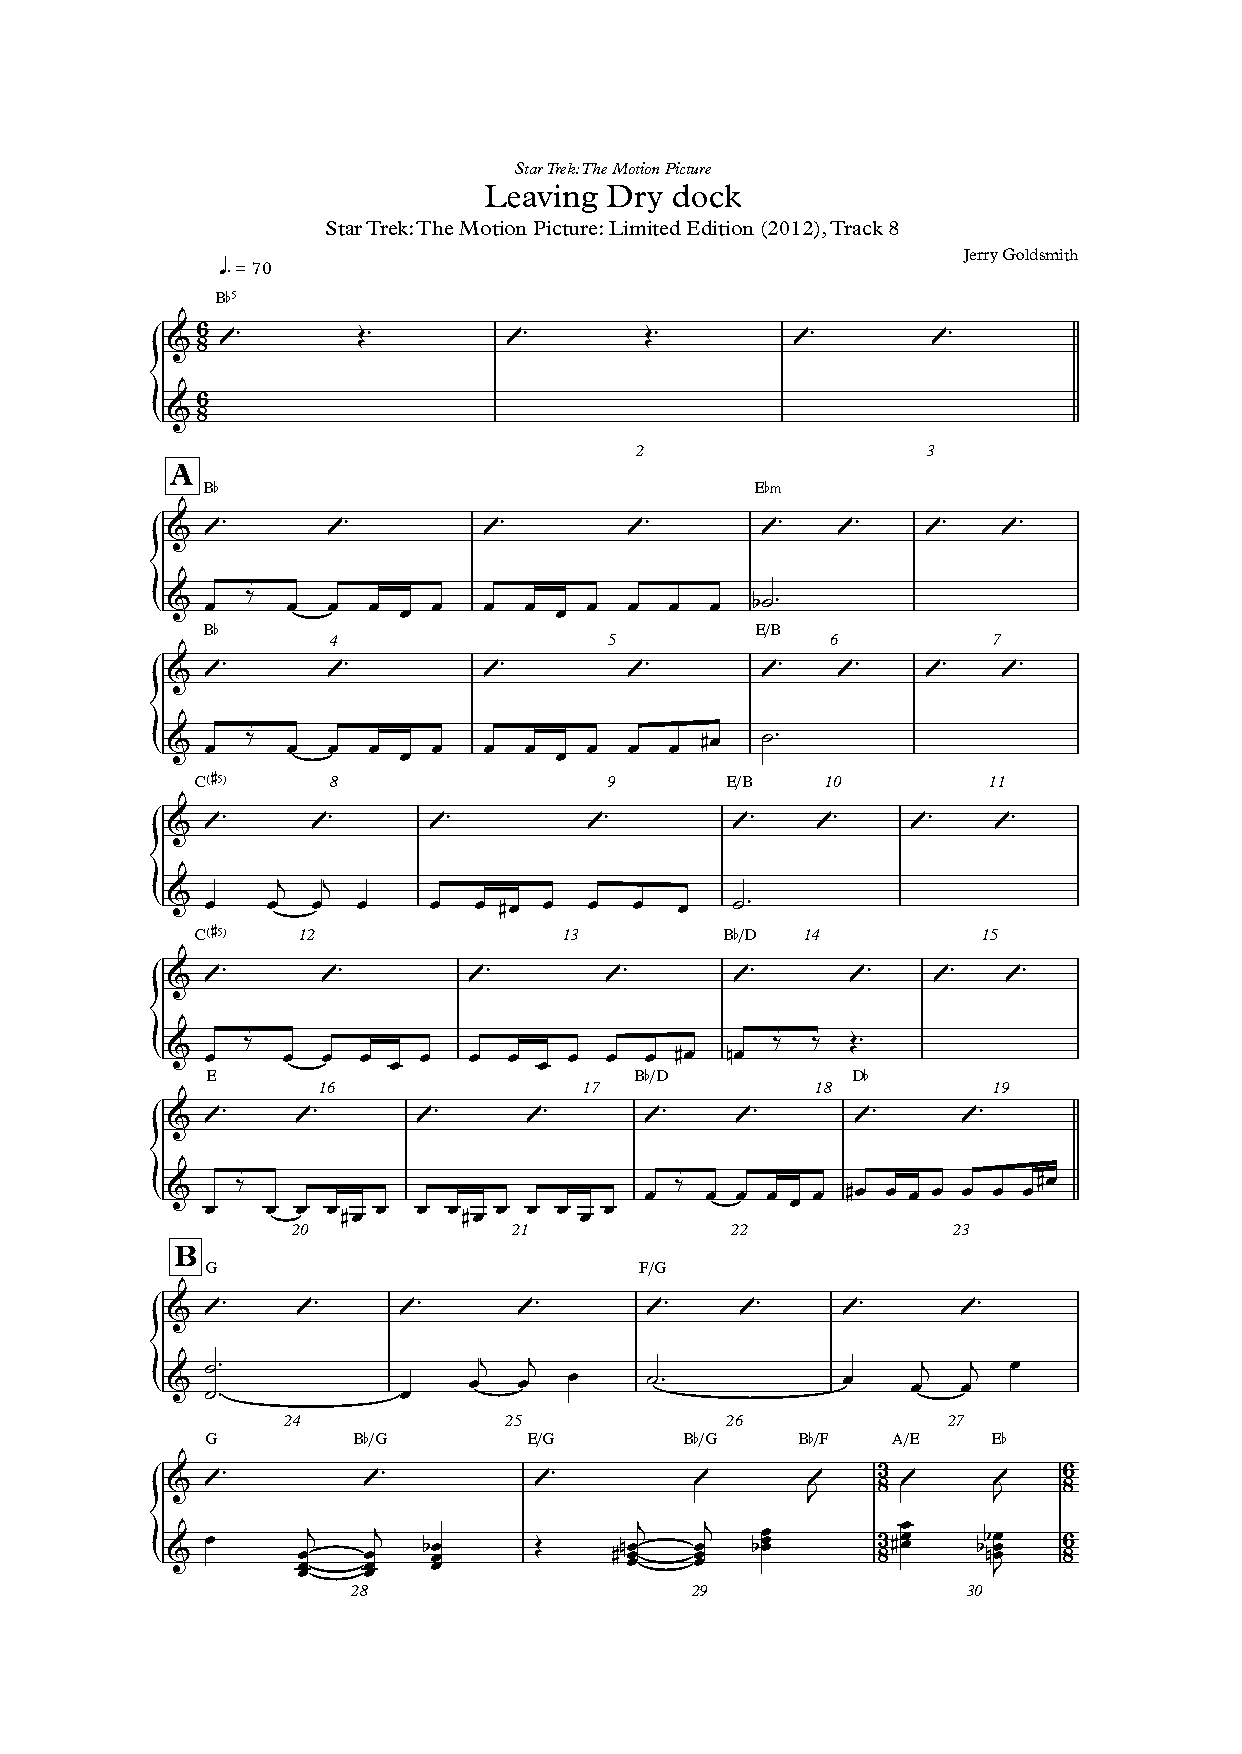
\includepdf[pages=-,pagecommand=\thispagestyle{fancy}]{pdf/st1/STTMP_Leaving_Drydock.pdf}

% Reviewed